\documentclass{beamer}
\usepackage[utf8]{inputenc}

\usetheme{Madrid}
\usecolortheme{default}
\usepackage{amsmath,amssymb,amsfonts,amsthm}
\usepackage{txfonts}
\usepackage{tkz-euclide}
\usepackage{listings}
\usepackage{adjustbox}
\usepackage{array}
\usepackage{tabularx}
\usepackage{gvv}
\usepackage{lmodern}
\usepackage{circuitikz}
\usepackage{tikz}
\usepackage{graphicx}
\usepackage{mathtools}
\setbeamertemplate{page number in head/foot}[totalframenumber]

\usepackage{tcolorbox}
\tcbuselibrary{minted,breakable,xparse,skins}



\definecolor{bg}{gray}{0.95}
\DeclareTCBListing{mintedbox}{O{}m!O{}}{%
  breakable=true,
  listing engine=minted,
  listing only,
  minted language=#2,
  minted style=default,
  minted options={%
    linenos,
    gobble=0,
    breaklines=true,
    breakafter=,,
    fontsize=\small,
    numbersep=8pt,
    #1},
  boxsep=0pt,
  left skip=0pt,
  right skip=0pt,
  left=25pt,
  right=0pt,
  top=3pt,
  bottom=3pt,
  arc=5pt,
  leftrule=0pt,
  rightrule=0pt,
  bottomrule=2pt,
  toprule=2pt,
  colback=bg,
  colframe=orange!70,
  enhanced,
  overlay={%
    \begin{tcbclipinterior}
    \fill[orange!20!white] (frame.south west) rectangle ([xshift=20pt]frame.north west);
    \end{tcbclipinterior}},
  #3,
}
\lstset{
    language=C,
    basicstyle=\ttfamily\small,
    keywordstyle=\color{blue},
    stringstyle=\color{orange},
    commentstyle=\color{green!60!black},
    numbers=left,
    numberstyle=\tiny\color{gray},
    breaklines=true,
    showstringspaces=false,
}

\title 
{1.5.39}
\date{August, 2025}


\author 
{Surya Sri - EE25BTECH11053}



\begin{document}


\frame{\titlepage}
\begin{frame}{Question}
The point ${R}$ divides the line segment $PQ$ in the ratio $3:1$ and $S$ is the midpoint of the line segment $PR$. Find the position vector of $S$ in terms of ${P}$ and ${Q}$.
\end{frame}



\begin{frame}{Variables used}
\begin{table}[H]    
  \centering
  \begin{tabular}[12pt]{ |c| c|}
    \hline
    \textbf{Vector} & \textbf{Matrix}\\ 
    \hline
	\begin{pmatrix}
p_1 \\
p_2 \\
p_3
\end{pmatrix} & P \\
    \hline 
	\begin{pmatrix}
q_1 \\
q_2 \\
q_3
\end{pmatrix} &  Q\\

    \hline
    \end{tabular}
  \caption{Variables Used}
  \label{tab:1.5.39}
\end{table}

\end{frame}

\begin{frame}{Solution}


The position vector of S in terms of P and Q is given completely in matrix form as follows:

Let

$$
\vec{P} =
\begin{pmatrix}
p_1 \\
p_2 \\
p_3
\end{pmatrix}
,
\quad
\vec{Q} =
\begin{pmatrix}
q_1 \\
q_2 \\
q_3
\end{pmatrix}
$$


\begin{align}
\vec{R} = \frac{3\vec{Q} + 1\vec{P}}{3 + 1} = \frac{3\vec{Q} + \vec{P}}{4}
\end{align}
So,
\begin{align}
\vec{R} =
\frac{1}{4}
\begin{pmatrix}
p_1 + 3q_1 \\
p_2 + 3q_2 \\
p_3 + 3q_3
\end{pmatrix}
\end{align}

\end{frame}

\begin{frame}{Solution}
    


Since S is the midpoint of PR,

\begin{align}
\vec{S} = \frac{\vec{P} + \vec{R}}{2}
\end{align}

\begin{align}
\vec{S} = \frac{1}{2} \left( \vec{P} + \frac{1}{4}(\vec{P} + 3\vec{Q}) \right )
\end{align}

\begin{align}
= \frac{1}{2} \left( \frac{4\vec{P} + \vec{P} + 3\vec{Q}}{4} \right )
= \frac{1}{2} \left( \frac{5\vec{P} + 3\vec{Q}}{4} \right )
= \frac{5\vec{P} + 3\vec{Q}}{8}
\end{align}


Therefore, the position vector of S is:

\begin{align}
\boxed{
\vec{S} =
\frac{1}{8}
\begin{pmatrix}
5p_1 + 3q_1 \\
5p_2 + 3q_2 \\
5p_3 + 3q_3
\end{pmatrix}
}
\end{align}


\end{frame}


\begin{frame}[fragile]
    \frametitle{Python}
    \begin{lstlisting}
import matplotlib.pyplot as plt

# Step 1: Assume coordinates for P and Q
P = (0, 0)
Q = (4, 0)

# Step 2: Find coordinates of R (divides PQ in ratio 3:1)
R_x = (3 * Q[0] + 1 * P[0]) / 4
R_y = (3 * Q[1] + 1 * P[1]) / 4
R = (R_x, R_y)

# Step 3: Find coordinates of S (midpoint of PR)
S_x = (P[0] + R[0]) / 2
S_y = (P[1] + R[1]) / 2
S = (S_x, S_y)

\end{lstlisting}
\end{frame}


\begin{frame}[fragile]
    \frametitle{Python}
    \begin{lstlisting}

# Step 4: Plot all points
plt.figure(figsize=(6, 4))
plt.plot([P[0], Q[0]], [P[1], Q[1]], 'k-', label='PQ')
plt.plot([P[0], R[0]], [P[1], R[1]], 'g--', label='PR')
plt.scatter(*P, color='blue', label='P (0,0)')
plt.scatter(*Q, color='red', label='Q (4,0)')
plt.scatter(*R, color='orange', label='R')
plt.scatter(*S, color='purple', label='S')

# Annotate points
plt.text(P[0], P[1]+0.2, 'P', ha='center')
plt.text(Q[0], Q[1]+0.2, 'Q', ha='center')
plt.text(R[0], R[1]+0.2, 'R', ha='center')
plt.text(S[0], S[1]+0.2, 'S', ha='center')


\end{lstlisting}
\end{frame}



\begin{frame}[fragile]
    \frametitle{Python}
    \begin{lstlisting}


plt.legend()
plt.grid(True)
plt.xlabel('x')
plt.ylabel('y')
plt.title('Points P, Q, R, S on Line Segment')
plt.axis('equal')
plt.savefig("graph.png") 
plt.show()


\end{lstlisting}
\end{frame}


\begin{frame}[fragile]
\frametitle{C Code}
\begin{lstlisting}
  
#include <stdio.h>

// For 2D vectors; change n to 3 for 3D.
#define n 2

void find_S(double P[], double Q[], double S[]) {
    // S = (5P + 3Q) / 8
    for (int i = 0; i < n; i++) {
        S[i] = (5 * P[i] + 3 * Q[i]) / 8.0;
    }
}

int main() {
    double P[n], Q[n], S[n];

 \end{lstlisting}
\end{frame} 


\begin{frame}[fragile]
\frametitle{C Code}
\begin{lstlisting}
    
    
    // Input coordinates for P and Q
    printf("Enter coordinates for P (x y): ");
    for (int i = 0; i < n; i++) scanf("%lf", &P[i]);

    printf("Enter coordinates for Q (x y): ");
    for (int i = 0; i < n; i++) scanf("%lf", &Q[i]);

    find_S(P, Q, S);

    printf("Coordinates of S: (%.3lf, %.3lf)\n", S[0], S[1]);
    return 0;
}

\end{lstlisting}
\end{frame}

\begin{frame}[fragile]
\frametitle{Python and C Code}

\begin{lstlisting}
 import subprocess

# Compile the C program
subprocess.run(["gcc", "points.c", "-o", "points"])

# Run the compiled C program
result = subprocess.run(["./points"], capture_output=True, text=True)

# Print the output from the C program (solution)
print(result.stdout) 

\end{lstlisting}
\end{frame}


\begin{frame}[fragile]
\frametitle{Graph}


\begin{figure}[H]
\begin{center}
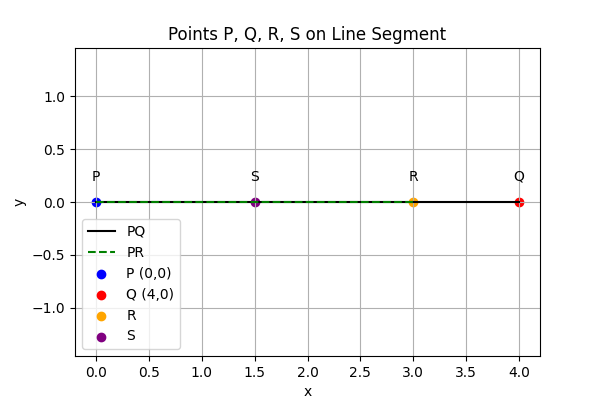
\includegraphics[width=0.75\columnwidth]{../figs/graph.png}
\end{center}
\caption{}
\label{fig:Fig}
\end{figure}



\end{frame}



\end{document}